\PassOptionsToPackage{unicode=true}{hyperref} % options for packages loaded elsewhere
\PassOptionsToPackage{hyphens}{url}
\documentclass[11pt,dvipsnames,ignorenonframetext,aspectratio=169]{beamer}
\IfFileExists{pgfpages.sty}{\usepackage{pgfpages}}{}
\setbeamertemplate{caption}[numbered]
\setbeamertemplate{caption label separator}{: }
\setbeamercolor{caption name}{fg=normal text.fg}
\beamertemplatenavigationsymbolsempty
\usepackage{lmodern}
\usepackage{amssymb,amsmath}
\usepackage{ifxetex,ifluatex}
\usepackage{fixltx2e} % provides \textsubscript
\ifnum 0\ifxetex 1\fi\ifluatex 1\fi=0 % if pdftex
  \usepackage[T1]{fontenc}
  \usepackage[utf8]{inputenc}
\else % if luatex or xelatex
  \ifxetex
    \usepackage{mathspec}
  \else
    \usepackage{fontspec}
\fi
\defaultfontfeatures{Ligatures=TeX,Scale=MatchLowercase}







\fi

  \usetheme[]{monash}

  \usecolortheme{monashwhite}


% A default size of 24 is set in beamerthememonash.sty

% Title page
\setbeamertemplate{title page}
{\placefig{-0.01}{-0.01}{width=1.01\paperwidth,height=1.01\paperheight}{weed.jpg}
\begin{textblock}{7.5}(1,2.8)\usebeamerfont{title}
{\color{white}\raggedright\par\inserttitle}
\end{textblock}
\begin{textblock}{7.5}(1,7)
{\color{white}\raggedright{\insertauthor}\mbox{}\\[0.2cm]
\insertdate}
\end{textblock}}


  \useinnertheme{rounded}

  \useoutertheme{smoothtree}

% use upquote if available, for straight quotes in verbatim environments
\IfFileExists{upquote.sty}{\usepackage{upquote}}{}
% use microtype if available
\IfFileExists{microtype.sty}{%
  \usepackage{microtype}
  \UseMicrotypeSet[protrusion]{basicmath} % disable protrusion for tt fonts
}{}


\newif\ifbibliography


\hypersetup{
      pdftitle={Global positioning system (GPS), components and its functions},
            colorlinks=true,
    linkcolor=red,
    citecolor=Blue,
    urlcolor=lightgrayd,
    breaklinks=true}
%\urlstyle{same}  % Use monospace font for urls







% Prevent slide breaks in the middle of a paragraph:
\widowpenalties 1 10000
\raggedbottom

  \AtBeginPart{
    \let\insertpartnumber\relax
    \let\partname\relax
    \frame{\partpage}
  }
  \AtBeginSection{
    \ifbibliography
    \else
      \let\insertsectionnumber\relax
      \let\sectionname\relax
      \frame{\sectionpage}
    \fi
  }
  \AtBeginSubsection{
    \let\insertsubsectionnumber\relax
    \let\subsectionname\relax
    \frame{\subsectionpage}
  }



\setlength{\parindent}{0pt}
\setlength{\parskip}{6pt plus 2pt minus 1pt}
\setlength{\emergencystretch}{3em}  % prevent overfull lines
\providecommand{\tightlist}{%
  \setlength{\itemsep}{0pt}\setlength{\parskip}{0pt}}

  \setcounter{secnumdepth}{0}


%% Monash overrides
\AtBeginSection[]{
   \frame<beamer>{
   \frametitle{Outline}\vspace*{0.2cm}
   
   \tableofcontents[currentsection,hideallsubsections]
  }}

% Redefine shaded environment if it exists (to ensure text is black)
\ifcsname Shaded\endcsname
  \definecolor{shadecolor}{RGB}{225,225,225}
  \renewenvironment{Shaded}{\color{black}\begin{snugshade}\color{black}}{\end{snugshade}}
\fi
%%


  \usepackage{setspace}
  \usepackage{wasysym}
  % \usepackage{footnote} % don't use this this breaks all
  \usepackage{fontenc}
  \usepackage{fontawesome}
  \usepackage{booktabs,siunitx}
  \usepackage{longtable}
  \usepackage{array}
  \usepackage{multirow}
  \usepackage{wrapfig}
  \usepackage{float}
  \usepackage{colortbl}
  \usepackage{pdflscape}
  \usepackage{tabu}
  \usepackage{threeparttable}
  \usepackage{threeparttablex}
  \usepackage[normalem]{ulem}
  \usepackage{makecell}
  \usepackage{xcolor}
  \usepackage{tikz} % required for image opacity change
  \usepackage[absolute,overlay]{textpos} % for text formatting
  \usepackage{chemfig}
  \usepackage[skip=0.333\baselineskip]{caption}
  % \newcommand*{\AlignChar}[1]{\makebox[1ex][c]{\ensuremath{\scriptstyle#1}}}%

  % this font option is amenable for beamer
  \setbeamerfont{caption}{size=\tiny}
  \singlespacing
  \definecolor{lightgrayd}{gray}{0.95}
  \definecolor{skyblued}{rgb}{0.65, 0.6, 0.94}
  \definecolor{oranged}{RGB}{245, 145, 200}

  % \newlength{\cslhangindent}
  % \setlength{\cslhangindent}{1.5em}
  % \newenvironment{cslreferences}%
  %   {\setlength{\parindent}{0pt}%
  %   \everypar{\setlength{\hangindent}{\cslhangindent}}\ignorespaces}%
  %   {\par}


  \newcommand{\bcolumns}{\begin{columns}[T, onlytextwidth]}
  \newcommand{\ecolumns}{\end{columns}}

  \newcommand{\bdescription}{\begin{description}}
  \newcommand{\edescription}{\end{description}}

  \newcommand{\bitemize}{\begin{itemize}}
  \newcommand{\eitemize}{\end{itemize}}
  \AtBeginSubsection{}

  \title[]{Global positioning system (GPS), components and its
functions}


  \author[
        \vspace{-0.5cm}Deependra Dhakal\\
Assistant Professor\\
\textit{ddhakal.rookie@gmail.com}\\
\url{https://rookie.rbind.io}
    ]{\vspace{-0.5cm}Deependra Dhakal\\
Assistant Professor\\
\textit{ddhakal.rookie@gmail.com}\\
\url{https://rookie.rbind.io}}


\date[
      
  ]{
    }

\begin{document}

% Hide progress bar and footline on titlepage
  \begin{frame}[plain]
  \titlepage
  \end{frame}


   \frame<beamer>{
   \frametitle{Outline}\vspace*{0.2cm}
   
   \tableofcontents[hideallsubsections]
  }

\hypertarget{global-positioning-system}{%
\section{Global positioning system}\label{global-positioning-system}}

\begin{frame}{}
\protect\hypertarget{section}{}
\begin{itemize}
\tightlist
\item
  Global navigation satellite system (GNSS) determines the location of
  field-observed reference data.
\item
  GNSS has applications in

  \begin{itemize}
  \tightlist
  \item
    navigating aircraft during sensor data acquisition
  \item
    geometrically correcting and referencing raw image data
  \end{itemize}
\item
  US Global Positioning System (GPS) was originally developed for
  military purposes, but soon became ubiquitous in many civil
  applications worldwide -- vehicle navigation, surveying, locaion based
  services and cellular phones.

  \begin{itemize}
  \tightlist
  \item
    The system consists of at least 24 satellite rotating around the
    earth in precisely known orbits
  \item
    Typically, these satellites revolve around the earth approximately
    once every 12 hours, at an altitude of approximately 20,200 km.
  \end{itemize}
\end{itemize}
\end{frame}

\begin{frame}{}
\protect\hypertarget{section-1}{}
\begin{itemize}
\tightlist
\item
  With their positions in space precisely known at all times, the
  satellites transmit time-encoded radio signals that are recorded by
  ground-based receivers and can be used to aid in positioning and
  navigation.
\item
  A comprehensive European GNSS constellation, \emph{Galileo} as well as
  the Russian \emph{GLONASS} and Chinese \emph{Compass} system are
  operational counterparts to the US GPS system.
\end{itemize}
\end{frame}

\begin{frame}{}
\protect\hypertarget{section-2}{}
\bcolumns
\column{0.6\textwidth}
\footnotesize

\begin{itemize}
\tightlist
\item
  The means by which GNSS signals are used to determine ground positions
  is called \emph{satellite ranging}.
\item
  Conceptually, it involves measuring the time required for signals
  transmitted by at least four satellites to reach the ground receiver.
\item
  Knowing that the signals travel at the speed of light
  (\(\mathrm{3 \times 8^8 m/sec}\) in vaccum), the distance from each
  satellite to the receiver can be computed using a form of
  three-dimensional triangulation.
\item
  GNSS measurements are potentially subject to sources of errors such as
  clock bias, uncertainties in the satellite orbits (satellite ephemeris
  errors) and errors due to atmospheric conditions.
\item
  In recent years, there have been efforts to improve the accuracy of
  GNSS positioning through the development of regional networks of
  high-precision base stations, generally referred to as satellite-based
  augmentation systems (SBAS).
\end{itemize}

\column{0.4\textwidth}

\begin{figure}
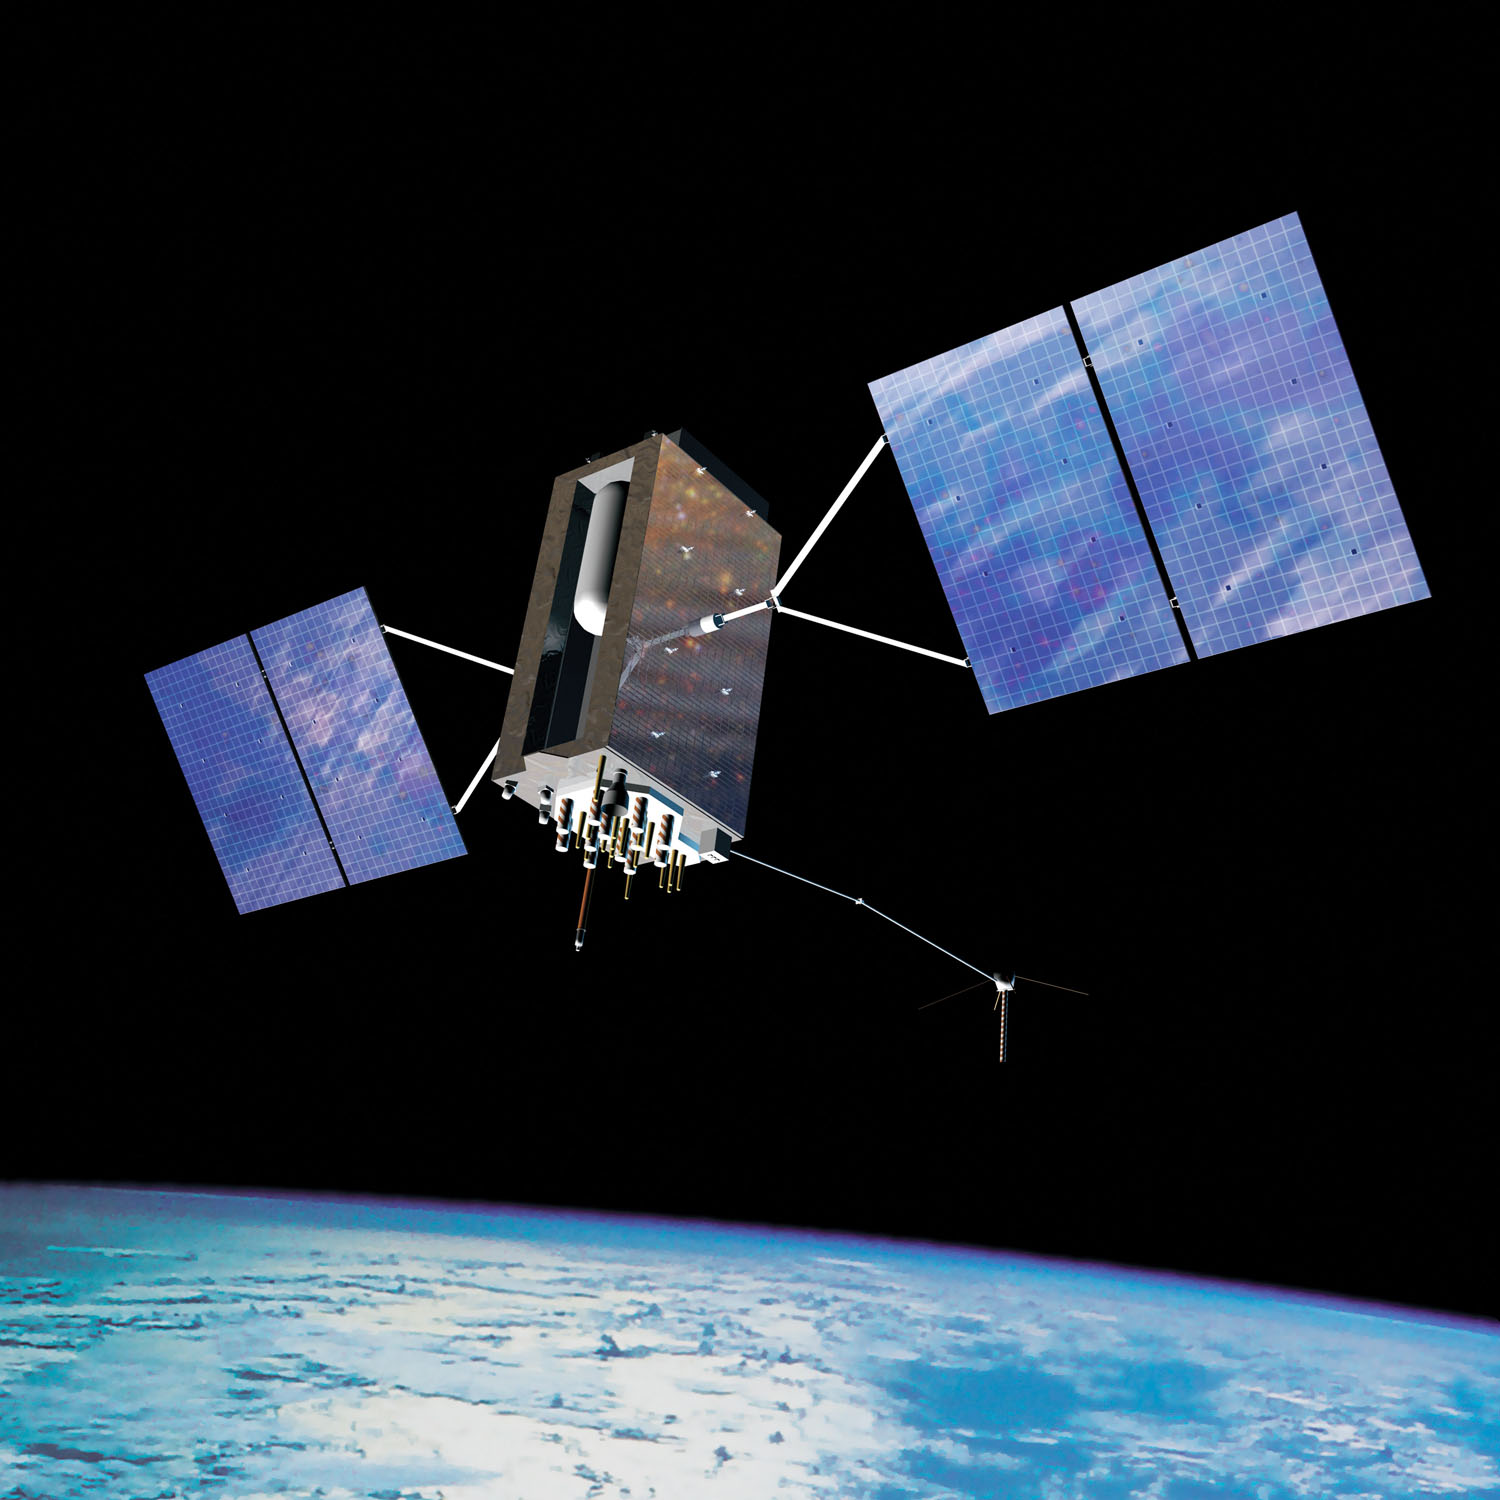
\includegraphics[width=0.72\linewidth]{../images/GPS_Block_IIIA} \caption{The U.S. Space Force's Global Positioning System was the first global satellite navigation system and was the first to be provided as a free global service. Source: \url{https://en.wikipedia.org/wiki/Satellite_navigation}}\label{fig:us-gps-satellite}
\end{figure}

\ecolumns
\end{frame}

\begin{frame}{}
\protect\hypertarget{section-3}{}
\bcolumns
\column{0.3\textwidth}

\begin{figure}
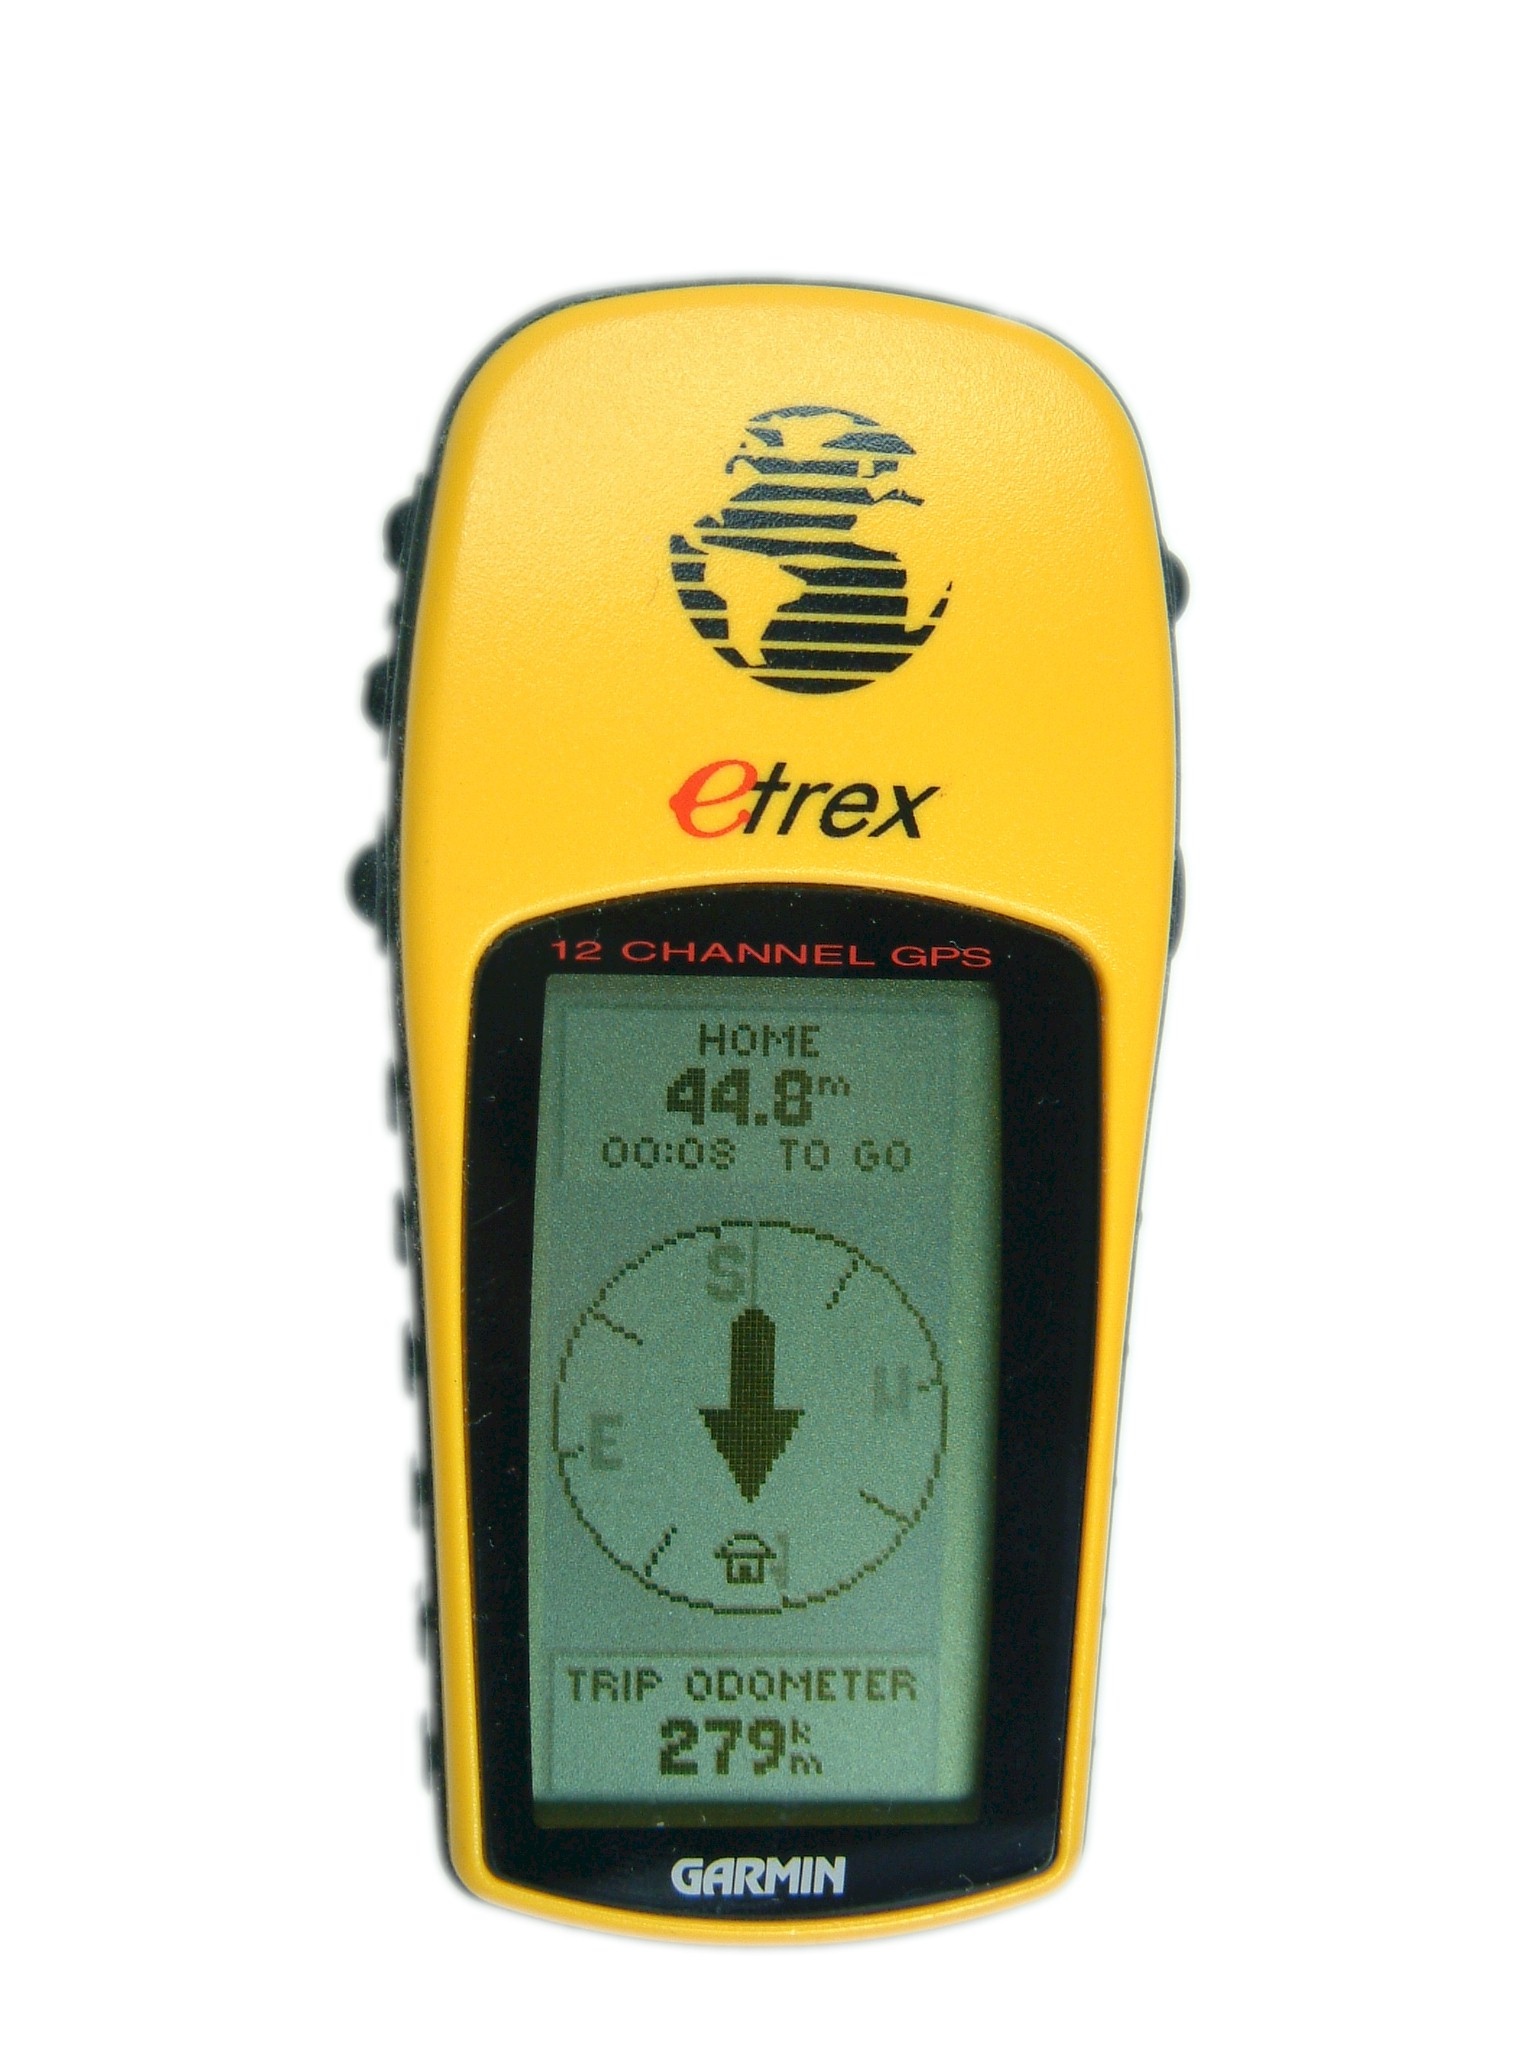
\includegraphics[width=0.4\linewidth]{../images/GPS_navigating_home} \end{figure}

\column{0.7\textwidth}
\small

\textbf{Applications of GPS navigation}

\begin{itemize}
\tightlist
\item
  Automobile
\item
  Air navigation usually having a moving map display and often connected
  to the autopilot for en-route navigation
\item
  Boats and ships (Maritime GNSS)
\item
  Construction and mining
\item
  Precision agriculture -- Agricultural equipment may use GNSS to steer
  automatically, or as a visual aid displayed on a screen for the
  driver. This is useful for controlled traffic and row crop operations
  and when spraying. Harvesters with yield monitors can also use GNSS to
  create a yield map.
\item
  Cycling and sports for touring and plotting the course
\item
  Exploration, hiking and climbing make use of GNSS to enable locating
  precisely in isolated areas.
\item
  Spacecraft GNSS
\end{itemize}

\ecolumns
\end{frame}

\hypertarget{bibliography}{%
\section{Bibliography}\label{bibliography}}

\begin{frame}{References}
\protect\hypertarget{references}{}
\end{frame}




\end{document}
